Since the presence of many processes have been reconciled at a theoretical
(even though abstract) level, here we will concentrate on fully spelled out
examples, in the simplest case of only two data points ($1$ and $2$) belonging
to two distinct processes.

Again, the following is in no way a proof, which has been spelled out in
details in \cref{sec:deriv}, for which considering more than two processes is
extremely relevant.

We will show the actual results of the obtained prescriptions for the
on-diagonal, $S_{11}$, and off-diagonal, $S_{12}$ cases.

Notice that, with respect to \cite{NNPDF:2019ubu}, here we have not yet
introduced the factor $s$, but it would still be allowed by \cref{eq:N-norm}.
In order to make the comparison with \cite{NNPDF:2019ubu} easier, in this
section we'll define the actual normalization including this factor, so: 
\begin{equation}
    N_m = \frac{m \cdot 3^{p-1}}{s_m}
\end{equation}

For convenience, the unnormalized shifts will be called $\delta$, i.e.:
\begin{equation}
    \delta_i(\vec{\kappa}) \equiv \Delta_i(\vec{\kappa}) \cdot \sqrt{N_m}
\end{equation}
In general, the expressions for the \textit{diagonal} and \textit{off-diagonal}
cases with only two process, $p = 2$, are the following:
\begin{description}
    \item[diagonal] effectively two-dimensional, since both the shifts depend only on two scales
        \begin{align}
            S_{11} &= \sum_{\vec{\kappa} \in \mathcal{V}} \Delta_1(\vec{\kappa}) \Delta_1(\vec{\kappa}) =\\
                   &= \frac{s_m}{3 \cdot m} \sum_{\vec{\kappa} \in \mathcal{V}_m^1} \delta_1(\vec{\kappa})^2 =\\
                   &= \frac{s_m}{m} \sum_{\substack{(\kappa_F, \kappa_{R,1}) \in v_m^1 }} \delta_1(\kappa_F, \kappa_{R, 1}, 0)^2
            \label{eq:main-explicit-diag}
        \end{align}
        where in the last step a single value has been chosen for $\kappa_{R,
        2}$, since $\delta_1$ does not depend on this scale.
    \item[off-diagonal] effectively three-dimensional, that only for this
        specific problem coincide with the whole space (for a greater number of
        processes, would be itself a projection)
        \begin{align}
            S_{12} &= \sum_{\vec{\kappa} \in \mathcal{V}} \Delta_1(\vec{\kappa}) \Delta_2(\vec{\kappa}) =\\
                   &= \frac{s_m}{3 \cdot m} \sum_{\vec{\kappa} \in \mathcal{V}_m^1\cap\mathcal{V}_m^2} \delta_1(\vec{\kappa}) \delta_2(\vec{\kappa})\\
                   &= \frac{s_m}{3 \cdot m} \sum_{\vec{\kappa} \in \mathcal{V}_m^1\cap\mathcal{V}_m^2} \delta_{12}(\vec{\kappa})
            \label{eq:main-off-diag}
        \end{align}
        where in the last step we defined $\delta_{12}(\vec{\kappa}) \equiv \delta_1(\vec{\kappa})\delta_2(\vec{\kappa})$.
\end{description}

\subsubsection{9 points}

The easiest prescription is the \textit{so-called} 9 points prescription,
because it corresponds to consider the whole two dimensional space as
$\mathcal{V}_9^i$, thus the two elements to be fixed are:
\begin{align}
    \label{eq:9specs}
    v_9 &= \{-, 0, +\}^2\\
    N_9 &= \frac{8 \cdot 3}{2} = 12
\end{align}
with $s_9 = 2$ (na\"ively because two scales are involved).

In the following, the expressions for the diagonal and off-diagonal cases are
formatted in order to stress the connection with the various pictures in this
section.
Concerning the \textit{diagonal} expressions they are formatted on three lines,
with three terms each, such that each term correspond to one point in the
two-dimensional diagram.
Since \textit{off-diagonal} would correspond to a three-dimensional picture,
this picture is ideally sliced in two-dimensional planes, and each plane is
displayed in the equation as a block of terms in square brackets, and slightly
indented with respect to previous blocks.
In order to preserve the shape, and to stress the effect of zero values in the
$c_i(\vec{\kappa})$, missing terms are explicitly marked with zeros.

\begin{description}
    \item[diagonal] for this prescription, we effectively have only 8 shifts,
        since out of the 9 theory predictions, one shift vanishes, just
        because it is used as the reference
        \begin{alignat}{4}
            S_{11} = \frac{1}{4} \bigg[ \nonumber
                &\delta_1(-,-,0)^2 &&+ \delta_1(-,0,0)^2 &&+ \delta_1(-,+,0)^2 &&+\\
                &\delta_1(0,-,0)^2 &&+ \qquad0 &&+ \delta_1(0,+,0)^2 &&+\\
                &\delta_1(+,-,0)^2 &&+ \delta_1(+,0,0)^2 &&+ \delta_1(+,+,0)^2
            \bigg] \nonumber
        \end{alignat}
    \item[off-diagonal] the two $\Delta_i$ combine in three dimensions: each
        one contains 3 zero elements (relative to the two dimensional central
        value), but the two are overlapping over the central point $(\kappa_F,
        \kappa_{R,1}, \kappa_{R,2}) = (0, 0, 0)$, leading to only 5 zero
        elements out of $3^3=27$ total elements, see \cref{fig:9}; thus the 22
        non-vanishing elements are the following:
        \vspace*{-30pt}
        \begin{align}
            S_{12} = \frac{1}{12} &
            \nonumber
            \begin{alignedat}{4}\\\\
                \bigg\{\bigg[
                    &\delta_{12}(-,-,-) &&+ \delta_{12}(-,-,0) &&+ \delta_{12}(-,-,+) &&+\\
                    &\delta_{12}(-,0,-) &&+ \delta_{12}(-,0,0) &&+ \delta_{12}(-,0,+) &&+\\
                    &\delta_{12}(-,+,-) &&+ \delta_{12}(-,+,0) &&+ \delta_{12}(-,+,+) 
            \bigg] &&+\\
        \end{alignedat}\\
        \nonumber\\
                                  &\qquad
                                  \begin{alignedat}{4}
                                      \bigg[
                    &\delta_{12}(0,-,-) &&+ \sOs &&+ \delta_{12}(0,-,+) &&+ \\
                    &\sOs &&+ \sOs &&+ \sOs &&+ \\
                    &\delta_{12}(0,+,-) &&+ \sOs &&+ \delta_{12}(0,+,+) 
                                  \bigg]&&+\\
                              \end{alignedat}\\
                              \nonumber\\
            \nonumber&\qquad\qquad
            \begin{alignedat}{4}
                \bigg[
                    &\delta_{12}(+,-,-) &&+ \delta_{12}(+,-,0) &&+ \delta_{12}(+,-,+) &&+\\
                    &\delta_{12}(+,0,-) &&+ \delta_{12}(+,0,0) &&+ \delta_{12}(+,0,+) &&+\\
                    &\delta_{12}(+,+,-) &&+ \delta_{12}(+,+,0) &&+ \delta_{12}(+,+,+) 
            \bigg]\bigg\}
            \end{alignedat}
        \end{align}
\end{description}

\begin{figure}
    \label{fig:9}
    \centering
        $\vcenter{\hbox{{\begin{tikzpicture}
\draw[->] (-1.5,0) -- (1.5,0);
\draw[->] (0,-1.5) -- (0,1.5);
\filldraw[black] (0,0) circle (2pt);
\filldraw[black] (-1,0) circle (2pt);
\filldraw[black] (0,-1) circle (2pt);
\filldraw[black] (1,0) circle (2pt);
\filldraw[black] (0,1) circle (2pt);
\filldraw[black] (-1,-1) circle (2pt);
\filldraw[black] (1,-1) circle (2pt);
\filldraw[black] (-1,1) circle (2pt);
\filldraw[black] (1,1) circle (2pt);
\node at (0.5,1.5) {$\kappa_r$};
\node at (1.9,0) {$\kappa_f$};
\end{tikzpicture}}
}}$
    \qquad
        $\vcenter{\hbox{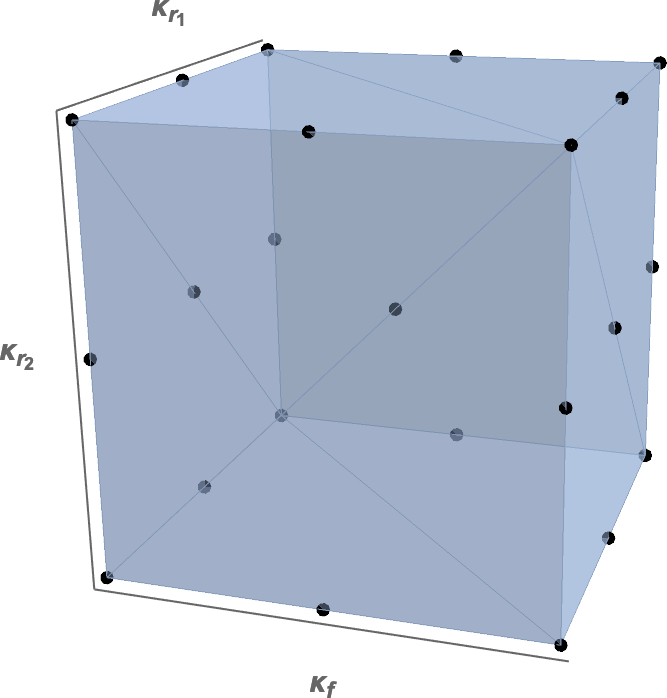
\includegraphics[width=0.3\textwidth]{ch-mhou/9-prescription}}}$
    \begin{caption}{
        Visualization of the 9 points prescription for the diagonal (2
        dimensional) and off-diagonal (3 dimensional) elements.
    }
    \end{caption}
\end{figure}

\subsubsection{5 points}

Another interesting prescription is the 5 points one, since it is a rather
minimal prescription involving both renormalization and factorization scale. 
\begin{align}
    \label{eq:5specs}
    v_5 &= \{(-, 0), (0, -), (+, 0), (0, +)\}\\
    N_5 &= \frac{4 \cdot 3}{2} = 6
\end{align}
with $s_5 = 2$ (same reason of \cref{eq:9specs}).

\begin{description}
    \item[diagonal] for this prescription, we effectively have only 4 shifts,
        since only 5 theory predictions are taken into account\footnote{
            with the shape of a Greek cross, as the $+$ symbol
        }, and, as for the 9 points, one is used as reference
        \begin{alignat}{4}
            S_{11} = \frac{1}{2} \bigg[ \nonumber
                &\sOs &&+ \delta_1(-,0,0)^2 &&+ \sOs &&+\\
                &\delta_1(0,-,0)^2 &&+ \sOs &&+ \delta_1(0,+,0)^2 &&+\\
                &\sOs &&+ \delta_1(+,0,0)^2 &&+ \sOs
            \bigg] \nonumber
        \end{alignat}
    \item[off-diagonal] in this case the two two-dimensional normalizations
        combine into one three-dimensional pattern, where non-zero elements are
        arranged in the shape of a double square pyramid: only central value is
        allowed for $\kappa_F \neq 0$, while the four corners are left for
        $\kappa_F = 0$ (same as the 9 points in this case), see \cref{fig:5}
        \vspace*{-30pt}
        \begin{align}
            S_{12} = \frac{1}{6} &
            \nonumber
            \begin{alignedat}{4}\\\\
                \bigg\{\bigg[
                    &\sOs &&+ \sOs &&+ \sOs &&+\\
                    &\sOs &&+ \delta_{12}(-,0,0) &&+ \sOs &&+\\
                    &\sOs &&+ \sOs &&+ \sOs 
                \bigg]&&+\\
            \end{alignedat}\\
            \nonumber\\
            &\qquad
            \begin{alignedat}{4}
                \bigg[
                    &\delta_{12}(0,-,-) &&+ \sOs &&+ \delta_{12}(0,-,+) &&+ \\
                    &\sOs &&+ \sOs &&+ \sOs &&+ \\
                    &\delta_{12}(0,+,-) &&+ \sOs &&+ \delta_{12}(0,+,+) 
                \bigg]&&+\\
            \end{alignedat}\\
            \nonumber\\
            \nonumber&\qquad\qquad
            \begin{alignedat}{4}
                \bigg[
                    &\sOs &&+ \sOs &&+ \sOs &&+\\
                    &\sOs &&+ \delta_{12}(+,0,0) &&+ \sOs &&+\\
                    &\sOs &&+ \sOs &&+ \sOs 
                \bigg]\bigg\}
            \end{alignedat}
        \end{align}
\end{description}

\begin{figure}
    \label{fig:5}
    \centering
        $\vcenter{\hbox{{\begin{tikzpicture}
\draw[->] (-1.5,0) -- (1.5,0);
\draw[->] (0,-1.5) -- (0,1.5);
\filldraw[black] (0,0) circle (2pt);
\filldraw[black] (-1,0) circle (2pt);
\filldraw[black] (0,-1) circle (2pt);
\filldraw[black] (1,0) circle (2pt);
\filldraw[black] (0,1) circle (2pt);
\node at (0.5,1.5) {$\kappa_r$};
\node at (1.9,0) {$\kappa_f$};
\end{tikzpicture}}
}}$
    \qquad
        $\vcenter{\hbox{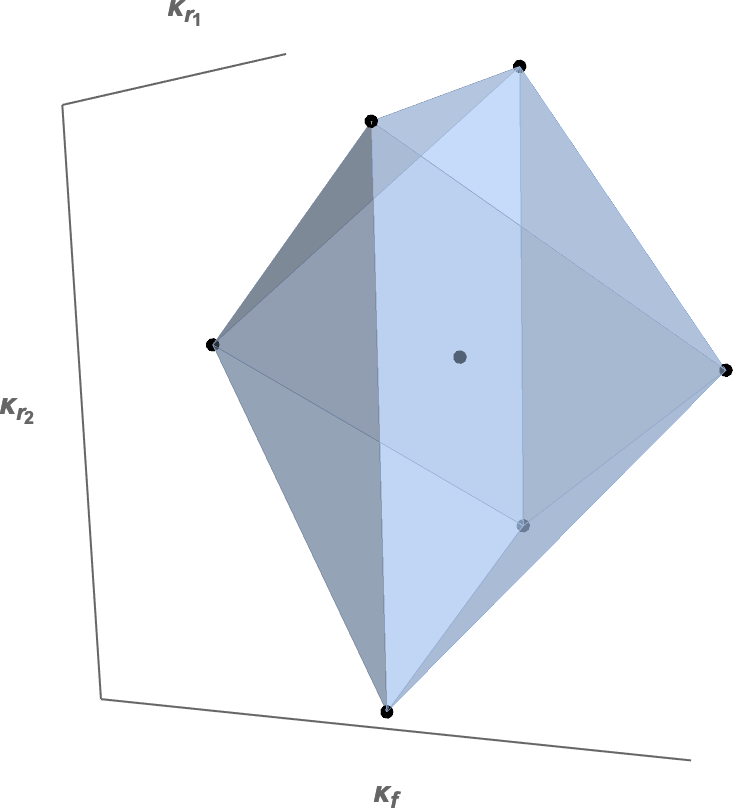
\includegraphics[width=0.3\textwidth]{ch-mhou/5-prescription}}}$
    \begin{caption}{
        Visualization of the 5 points prescription for the diagonal (2
        dimensional) and off-diagonal (3 dimensional) elements.
    }
    \end{caption}
\end{figure}

\subsubsection{$\bar{5}$ points}

Just another option with renormalization and factorization scale, with same two
dimensional volume, but a different geometry.
\begin{align}
    v_5 &= \{(-, -), (-, +), (+, -), (+, +)\}\\
    N_5 &= \frac{4 \cdot 3}{2}  = 6
\end{align}
with $s_{\bar{5}} = 2$ (same reason of \cref{eq:9specs}).

\begin{description}
    \item[diagonal] for this prescription, we effectively have only 4 shifts,
        since only 5 theory predictions are taken into account\footnote{
            with the shape of St. Andrew's cross, as the $\times$ symbol
        }, and, as for the 9 points, one is used as reference
        \begin{alignat}{4}
            S_{11} = \frac{1}{2} \bigg[ \nonumber
                &\delta_1(-,-,0)^2 &&+ \sOs &&+ \delta_1(-,+,0)^2 &&+\\
                &\sOs &&+ \qquad0 &&+ \sOs &&+\\
                &\delta_1(+,-,0)^2 &&+ \sOs &&+ \delta_1(+,+,0)^2
            \bigg] \nonumber
        \end{alignat}
    \item[off-diagonal] also in this case the two two-dimensional
        normalizations $c_i(\vec{\kappa})$ have the combined effect of setting
        to zero a lot of elements in the three dimensional space, this leaving
        the shape of an empty cube: the four corners are now left for $\kappa_F
        \neq 0$, and no point is left for $\kappa_F = 0$
        \vspace*{-30pt}
        \begin{align}
            S_{12} = \frac{1}{6} &
            \nonumber
            \begin{alignedat}{4}\\\\
                \bigg\{\bigg[
                    &\delta_{12}(-,-,-) &&+ \sOs &&+ \delta_{12}(-,-,+) &&+\\
                    &\sOs &&+ \sOs &&+ \sOs &&+\\
                    &\delta_{12}(-,+,-) &&+ \sOs &&+ \delta_{12}(-,+,+) 
            \bigg] &&+\\
        \end{alignedat}\\
        \nonumber\\
            &\qquad
            \begin{alignedat}{4}
                \bigg[
                    &\sOs &&+ \sOs &&+ \sOs &&+ \\
                    &\sOs &&+ \sOs &&+ \sOs &&+ \\
                    &\sOs &&+ \sOs &&+ \sOs 
                \bigg]&&+\\
            \end{alignedat}\\
            \nonumber\\
            \nonumber&\qquad\qquad
            \begin{alignedat}{4}
                \bigg[
                    &\delta_{12}(+,-,-) &&+ \sOs &&+ \delta_{12}(+,-,+) &&+\\
                    &\sOs &&+ \sOs &&+ \sOs &&+\\
                    &\delta_{12}(+,+,-) &&+ \sOs &&+ \delta_{12}(+,+,+) 
            \bigg]\bigg\}
            \end{alignedat}
        \end{align}
\end{description}

\begin{figure}
    \label{fig:5bar}
    \centering
        $\vcenter{\hbox{{\begin{tikzpicture}
\draw[->] (-1.5,0) -- (1.5,0);
\draw[->] (0,-1.5) -- (0,1.5);
\filldraw[black] (0,0) circle (2pt);
\filldraw[black] (-1,-1) circle (2pt);
\filldraw[black] (1,1) circle (2pt);
\filldraw[black] (1,-1) circle (2pt);
\filldraw[black] (-1,1) circle (2pt);
\node at (0.5,1.5) {$\kappa_r$};
\node at (1.9,0) {$\kappa_f$};
\end{tikzpicture}}
}}$
    \qquad
        $\vcenter{\hbox{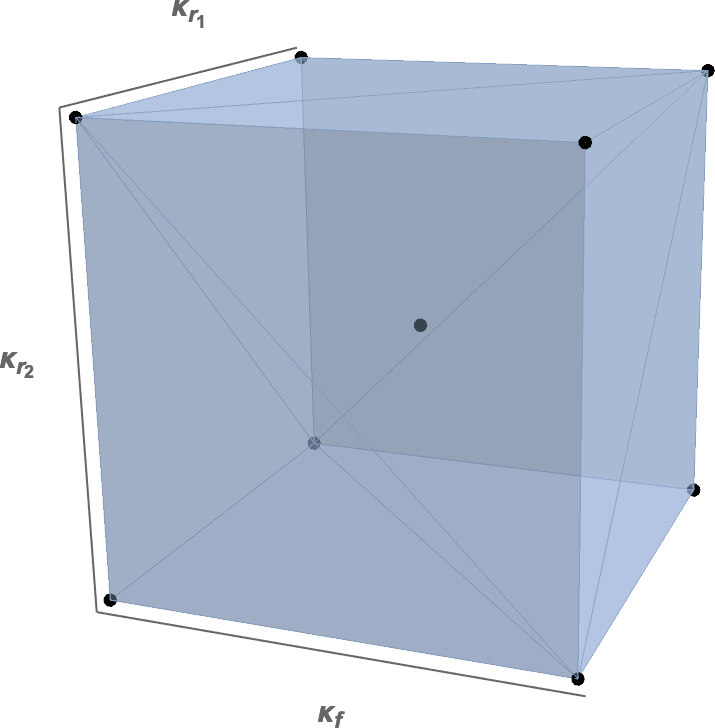
\includegraphics[width=0.3\textwidth]{ch-mhou/5bar-prescription}}}$
    \begin{caption}{
        Visualization of the $\bar{5}$ points prescription for the diagonal (2
        dimensional) and off-diagonal (3 dimensional) elements.
    }
    \end{caption}
\end{figure}
